\documentclass[a4paper]{article}
\usepackage{amsmath}
\usepackage{amssymb}
\usepackage{graphicx}
\usepackage{a4wide}
\usepackage{url}
\usepackage{pdfpages}

\usepackage{natbib} 
\citestyle{aa}
\bibpunct{(}{)}{;}{a}{}{,}

\newcommand{\mytilde}{\raise.17ex\hbox{$\scriptstyle\mathtt{\sim}$}}
\setlength{\parindent}{0pt}

% Listings to import code into LaTeX
\usepackage{listings}
\usepackage{color}
\usepackage{textcomp}
\definecolor{listinggray}{gray}{0.9}
\definecolor{lbcolor}{rgb}{0.9,0.9,0.9}
\lstset{
	backgroundcolor=\color{lbcolor},
	tabsize=4,
	rulecolor=,
	language=bash,
        basicstyle=\scriptsize,
        upquote=true,
        aboveskip={1.5\baselineskip},
        columns=fixed,
        showstringspaces=false,
        extendedchars=true,
        breaklines=true,
        prebreak = \raisebox{0ex}[0ex][0ex]{\ensuremath{\hookleftarrow}},
        frame=single,
        showtabs=false,
        showspaces=false,
        showstringspaces=false,
        identifierstyle=\ttfamily,
        keywordstyle=\color[rgb]{0,0,1},
        commentstyle=\color[rgb]{0.133,0.545,0.133},
        stringstyle=\color[rgb]{0.627,0.126,0.941},
}
% End of Listings

\begin{document}
\begin{figure}[h!] 
\begin{center} 

\includegraphics{UvA_Logo_Image_EN.jpg} \\

\includegraphics{UvA_Logo_Text_EN.jpg} \\

\includegraphics{API_Logo_Text.pdf} 
\end{center} 
\end{figure} 

\begin{center}
\line(1,0){420} \\
\huge \textbf{Basic Linux and Coding for AA (BLAC) \\ Exercise 5 (week 3)} \\
\line(1,0){420}
\end{center}

\vfill

%\begin{figure}[h!] 
%\begin{center} 
%\includegraphics[width=12cm]{graphgraphMyGraph} 
%\end{center} 
%\end{figure} 
%\addtocounter{figure}{-1} % start counting at figure 1 again


\begin{table}[h]
\begin{center}
\begin{tabular}{lp{5cm}l}
\textit{Author:} & & \emph{Supervisor:} \\
Timo Halbesma, 6126561 & & Dr. T. Coenen\\
\end{tabular}
\end{center}
\end{table}

% End of titlepage

\newpage

\section{Questions}
\begin{enumerate}
\item
The wettest day was at 19750623 in ROTTERDAM(344). The precipitation amount was 101.4 mm. \\
The hottest day was at 19760703 in VOLKEL(375). The temperature was 36.7 degrees Centigrade. \\
\item
Maximum temperature for station 260 in 1968 has the following first ten entries:\\
$[[260, 19680101, 23], [260, 19680102, 22], [260, 19680103, 27], [260, 19680104, 29],$ \\
$[260, 19680105, 84], [260, 19680106, 51], [260, 19680107, 22], [260, 19680108, 35],$\\
$[260, 19680109, -35], [260, 19680110, 32]]$

\item
I have chosen to plot the Maximum Temperature `TX' because the question did not specify which of the three temperature entries in the dataset should be used. Changing this is just a matter of changing one parameter in the function call though.
\begin{figure}[h!] 
\begin{center} 
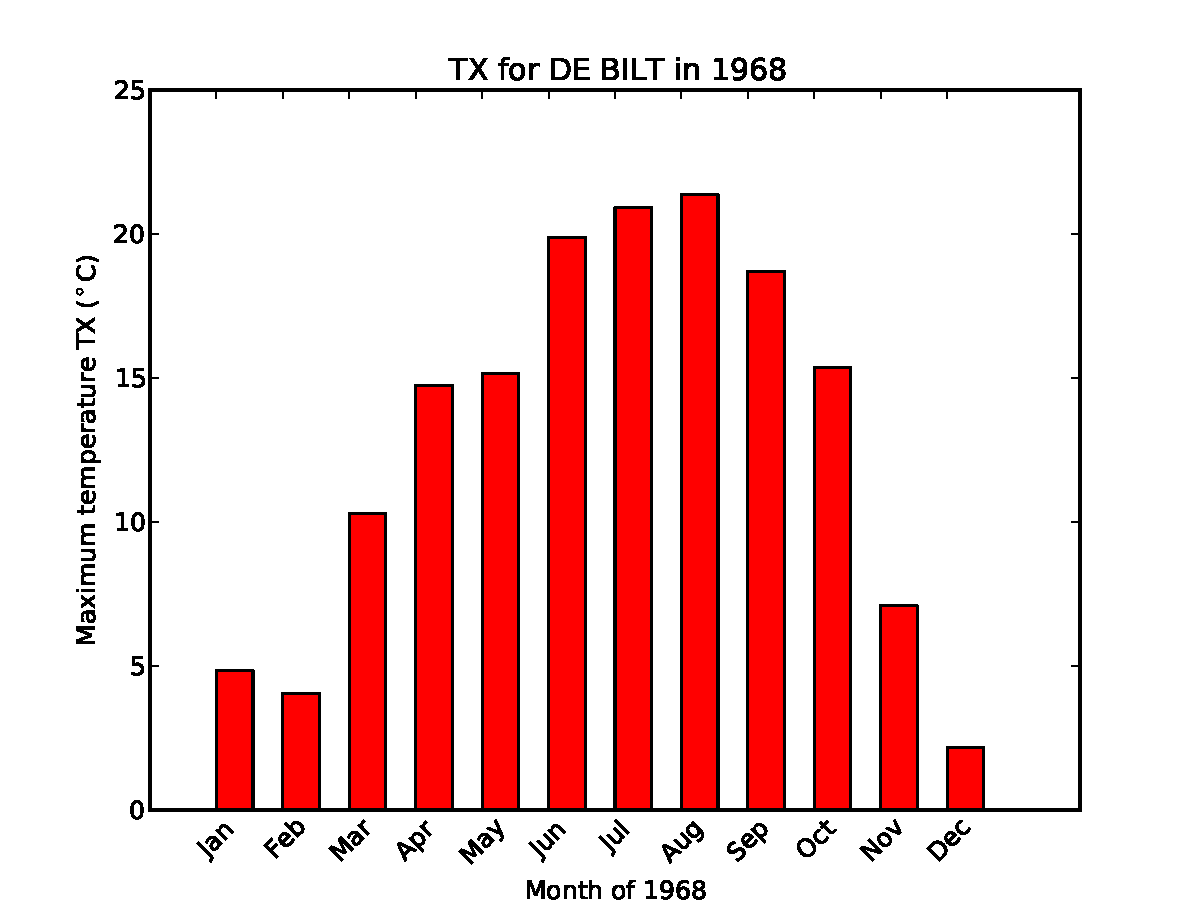
\includegraphics[scale=0.5]{../Week3/BLAC_hw5_TLRH_6126561_260_TX_1968.pdf} 
\caption{Required plot for third question.}
\end{center} 
\end{figure} 
\newpage
\item
From Figure~\ref{fig:summer} and Figure~\ref{fig:winter} it is clear that the summers in the station in the West (210, Valkenburg) are significantly hotter than in the East (283, Hupsel) in the period 1991 - 1996. Futhermore the winters in the East (283, Hupsel) are significantly colder than in the West (210, Valkenburg) in the same time period.
\begin{figure}[h!] 
\begin{center} 
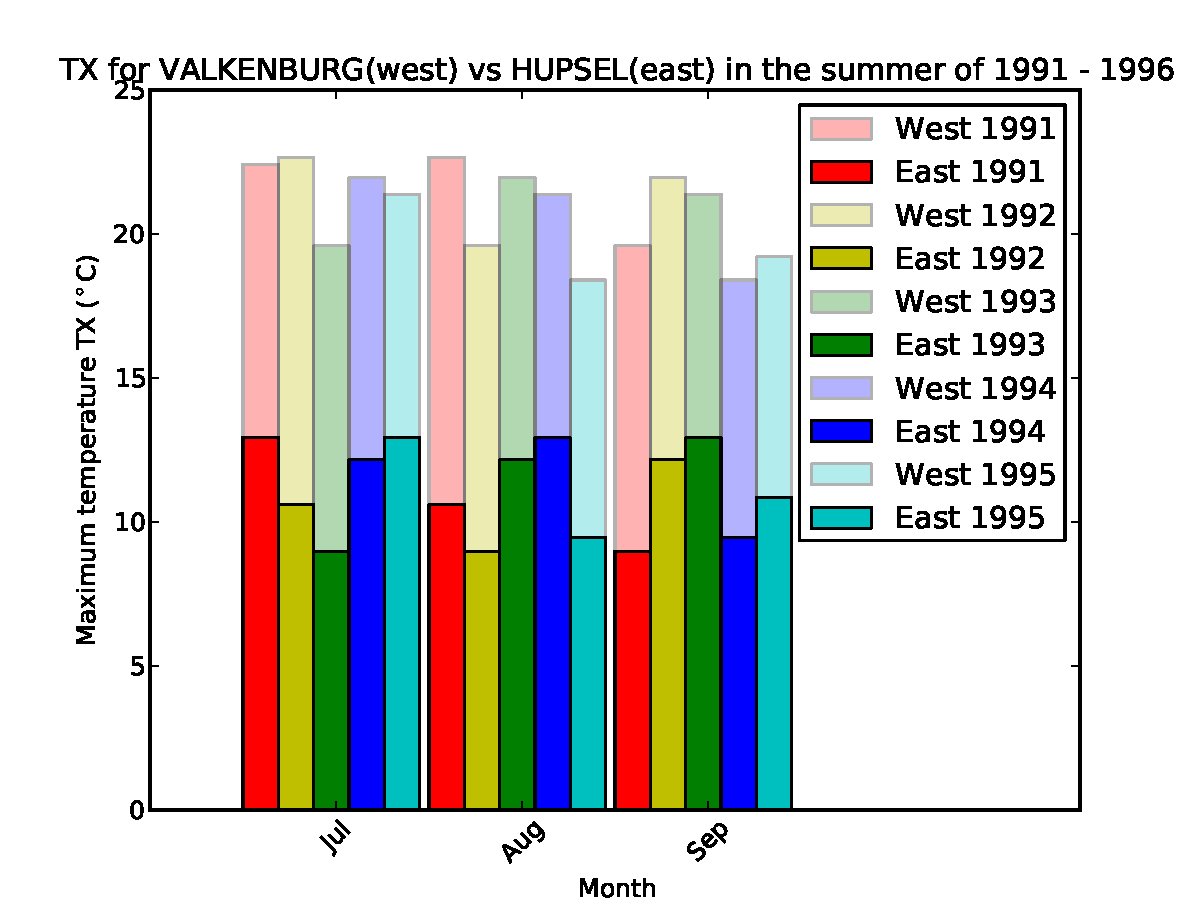
\includegraphics[scale=0.5]{../Week3/BLAC_hw5_TLRH_6126561_210vs283_TX_summer_1991.pdf} 
\caption{Maximum temperature in the summer for station Valkenburg (210) in the West versus station Hupsel (283) in the East.\label{fig:summer}}
\end{center} 
\end{figure} 

\begin{figure}[h!] 
\begin{center} 
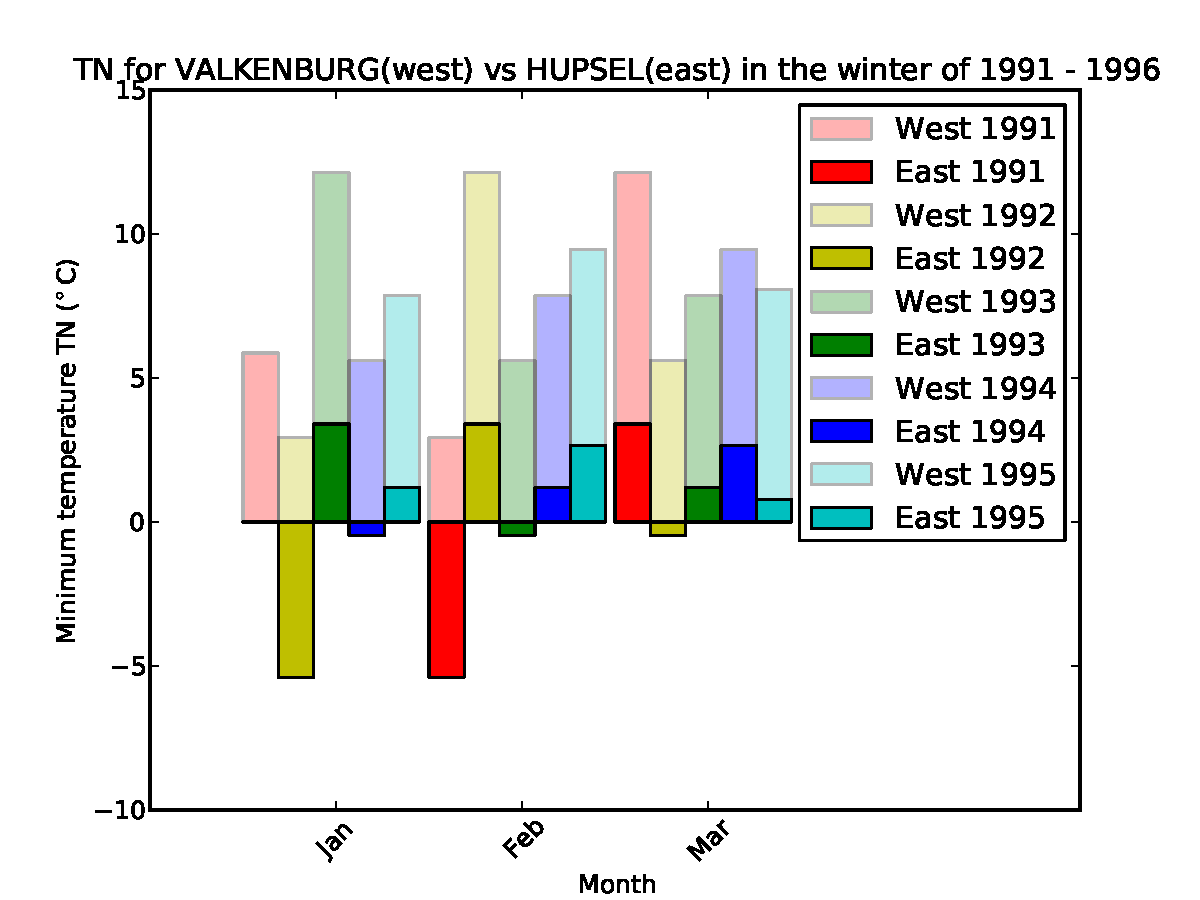
\includegraphics[scale=0.5]{../Week3/BLAC_hw5_TLRH_6126561_210vs283_TN_winter_1991.pdf} 
\caption{Minimum temperature in the winter for station Valkenburg (210) in the West versus station Hupsel (283) in the East..\label{fig:winter}}
\end{center} 
\end{figure} 

\item

\begin{figure}[h!] 
\begin{center} 
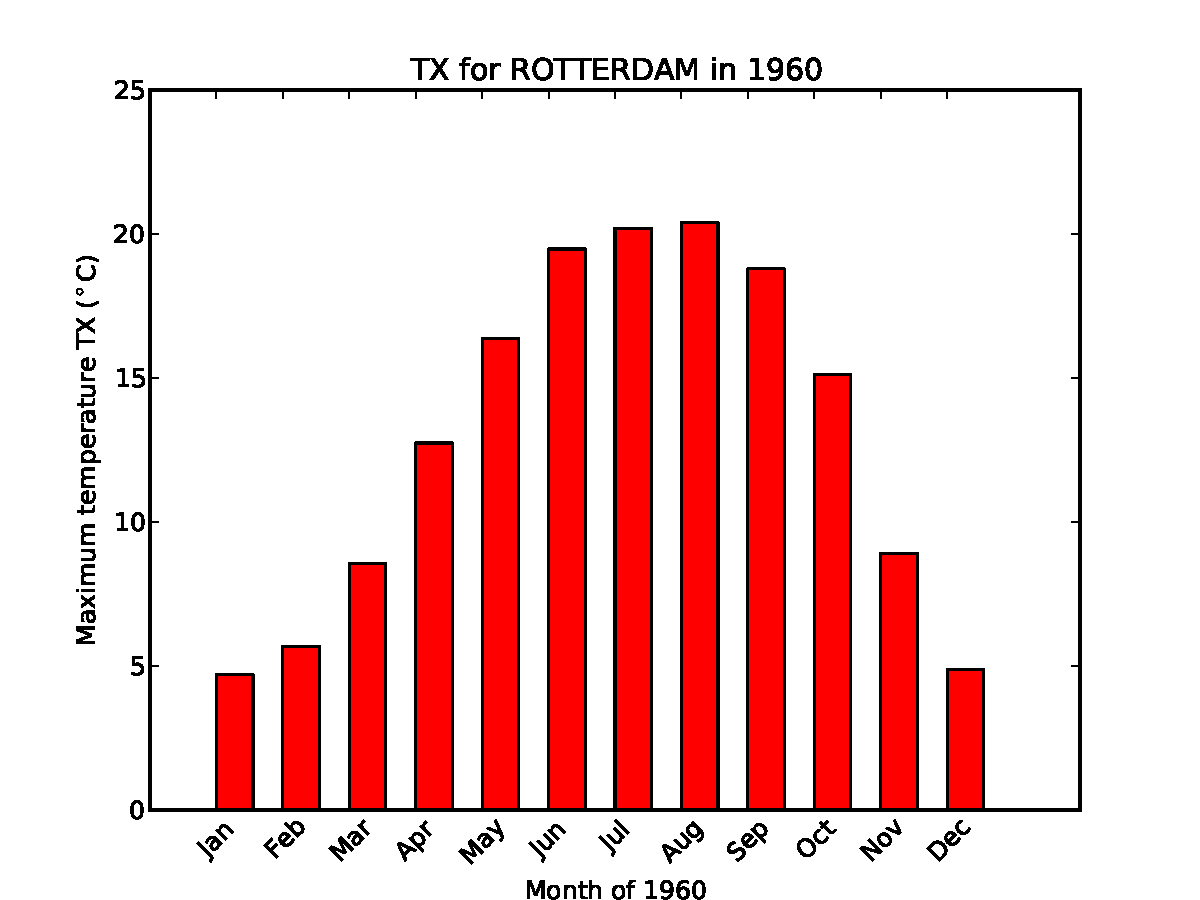
\includegraphics[scale=0.5]{../Week3/BLAC_hw5_TLRH_6126561_344_TX_1960.pdf} 
\caption{Monthly averaged decade 1960 - 1969 for station Rotterdam (344).}
\end{center} 
\end{figure} 

\item This homework set has taken quite a lot of time... skipping this one :-(

\end{enumerate}

\newpage

\lstinputlisting[caption={TLRH's solution for the BLAC homework 3 (week 2) \label{list:hw1}. Not that this code has been slightly modified since my last submission.}]{../Week2/knmi_1_6126561.py}

\lstinputlisting[caption={TLRH's solution for the BLAC homework 4 and 5 (week 2 and 3) \label{list:hw2}}]{../Week2/knmi_6126561.py}
\end{document}